\documentclass[logo,reportComp]{thesis}
\usepackage[cpp,pseudo]{mypackage}

\title{高级编程技术实验报告}
\subtitle{实验四:模拟疾病传播}
\school{数据科学与计算机学院}
\author{陈鸿峥}
\classname{17大数据与人工智能}
\stunum{17341015}
\headercontext{高级编程技术实验报告}
\lstset{language=python}

\begin{document}

\maketitle

\section{问题描述及求解思路}
\subsection{实现无抗生素模拟}
\verb'SimpleBacteria'类
\begin{itemize}
	\item \verb'__init__':直接设置\verb'birth_prob'和\verb'death_prob'
	\item \verb'is_killed':生成随机数\verb'random.random()',如果小于死亡率,则意味着已经死了
	\item \verb'reproduce':生成随机数\verb'random.random()',如果小于\verb'self.birth_prob * (1 - pop_density)',则返回一个新的\verb'SimpleBacteria'实例,否则\verb'raise NoChildException'
\end{itemize}

\verb'Patient'类
\begin{itemize}
	\item \verb'__init__':直接设置\verb'bacteria'和\verb'max_pop'
	\item \verb'get_total_pop':返回\verb'self.bacteria'的长度
	\item \verb'update':按照代码注释的步骤一步一步模拟即可
\begin{lstlisting}
def update(self):
    new_bacteria = []
    for bact in self.bacteria:
        if not bact.is_killed():
            new_bacteria.append(bact)
    # calculate current population density
    curr_pop_density = len(new_bacteria) / self.max_pop
    # determine which bacteria will reproduce
    new_offspring = []
    for bact in new_bacteria:
        try:
            new_offspring.append(bact.reproduce(curr_pop_density))
        except: # NoChild!
            pass
    # merge results
    new_bacteria += new_offspring
    self.bacteria = new_bacteria
    return self.get_total_pop()
\end{lstlisting}
\end{itemize}

\subsection{运行分析无抗生素模拟}
\verb'calc_pop_avg'取时间步$n$的所有模拟,并计算平均值。
\begin{lstlisting}
def calc_pop_avg(populations, n):
    avg = 0.
    num_trials = len(populations)
    for i in range(num_trials):
        avg += populations[i][n]
    return avg / num_trials
\end{lstlisting}

\verb'simulation_without_antibiotic'对于每一次尝试,先初始化\verb'SimpleBacteria'和\verb'Patient'的实例,然后对于每一个时间步对\verb'Patient'实例进行\verb'update'操作,并将该轮细胞数记录在数组中。
具体实施如下。
\begin{lstlisting}
def simulation_without_antibiotic(num_bacteria, max_pop, birth_prob, death_prob, num_trials):
    num_time_steps = 300
    populations = []
    for trail in range(num_trials):
        # initialization
        populations.append([])
        bacteria = []
        for i in range(num_bacteria):
            bacteria.append(SimpleBacteria(birth_prob,death_prob))
        patient = Patient(bacteria,max_pop)
        # simulation
        for t in range(num_time_steps):
            populations[trail].append(patient.update())
    # calculate average populations
    avg_pop = []
    for t in range(num_time_steps):
        avg_pop.append(calc_pop_avg(populations,t))
    # plot results
    make_one_curve_plot(
        range(num_time_steps),
        avg_pop,
        "Timestep",
        "Average Population",
        "Without Antibiotic"
    )
    return populations
\end{lstlisting}

运行结果见图\ref{fig:p2}。

\subsection{计算置信区间}
依照下述公式计算即可
\[\begin{aligned}
\bar{x}&=\frac{1}{n}\sum_{i=1}^nx_i\\
\sigma&=\sqrt{\frac{1}{n}\sum_{i=1}^n(x_i-\bar{x})^2}\\
\text{SEM}&=\frac{\sigma}{\sqrt{n}}\\
\text{CondInt}&=\bar{x}\pm 1.96(\text{SEM})
\end{aligned}\]

注意由于Python没有内置\verb'sqrt'函数,故只有计算平方根的位置调用了\verb'numpy'包(当然用内置\verb'math'库也是可以的)。
测试结果见图\ref{fig:test}。
\begin{lstlisting}
def calc_pop_std(populations, t):
    num_trials = len(populations)
    avg_pop = calc_pop_avg(populations,t)
    sigma = 0
    for i in range(num_trials):
        sigma += (populations[i][t] - avg_pop)**2
    return np.sqrt(sigma / num_trials)

def calc_95_ci(populations, t):
    num_trials = len(populations)
    mean = calc_pop_avg(populations,t)
    SEM = calc_pop_std(populations,t) / np.sqrt(num_trials)
    width = 1.96 * SEM
    return (mean, width)
\end{lstlisting}

并在问题二\verb'# plot results'的代码前面加上下面两条语句,即可输出置信区间
\begin{lstlisting}
mean, width = calc_95_ci(populations,299)
print("95% confidence interval: [{:.4},{:.4}]".format(mean-width,mean+width))
\end{lstlisting}

运行结果第\ref{sub:results}节分析。

\subsection{实现有抗生素模拟}
\verb'ResistantBacteria'类
\begin{itemize}
	\item \verb'__init__':利用父类构造函数\verb'SimpleBacteria.__init__(self,birth_prob,death_prob)'初始化,同时也要初始化\verb'resistant'和\verb'mut_prob'
	\item \verb'get_resistant':返回\verb'self.resistant'
	\item \verb'is_killed':先判断是否有抵抗性,如果有则以\verb'self.death_prob'作为死亡率,否则以\verb'self.death_prob / 4'作为死亡率。判断是否死亡的方法同\verb'SimpleBacteria'。
	\item \verb'reproduce':注意处理好各个状态之间的关系,先判断是否繁衍,然后才判断是否有抵抗性,最后判断是否变异
\begin{lstlisting}
if random.random() < self.birth_prob * (1 - pop_density):
    if self.resistant:
        return ResistantBacteria(self.birth_prob,self.death_prob,True,self.mut_prob)
    elif random.random() < self.mut_prob * (1 - pop_density):
        return ResistantBacteria(self.birth_prob,self.death_prob,True,self.mut_prob)
    else:
        return ResistantBacteria(self.birth_prob,self.death_prob,False,self.mut_prob)
else:
    raise NoChildException
\end{lstlisting}
\end{itemize}

\verb'TreatedPatient'类
\begin{itemize}
	\item \verb'__init__':设置\verb'self.on_antibiotic'为假,然后调用父类构造函数\verb'Patient.__init__(self,bacteria,max_pop)'进行初始化
	\item \verb'set_on_antibiotic':设置\verb'self.on_antibiotic'为真
	\item \verb'get_resist_pop':枚举每一个细菌,如果有抵抗性则计数加1,最后返回有抵抗性的细菌总数
	\item \verb'update':按照代码注释的步骤一步一步模拟即可,下面\verb'NEW'的部分是\verb'TreatedPatient'特有的
\begin{lstlisting}
def update(self):
    # determine whether bacteria dies
    new_bacteria = []
    for bact in self.bacteria:
        if not bact.is_killed():
            new_bacteria.append(bact)
    # (NEW!) determine if the patient is on antibiotics
    if self.on_antibiotic:
        res_bacteria = []
        for bact in new_bacteria:
            if bact.get_resistant():
                res_bacteria.append(bact)
        # update new bacteria
        new_bacteria = res_bacteria
    # calculate current population density
    curr_pop_density = len(new_bacteria) / self.max_pop
    new_offspring = []
    for bact in new_bacteria:
        try:
            new_offspring.append(bact.reproduce(curr_pop_density))
        except:
            pass
    # merge results
    new_bacteria += new_offspring
    self.bacteria = new_bacteria
    return self.get_total_pop()
\end{lstlisting}
\end{itemize}

\subsection{运行分析有抗生素模拟}
\verb'simulation_without_antibiotic'对于每一次尝试,先初始化\verb'SimpleBacteria'和\verb'Patient'的实例,然后对于每一个时间步对\verb'Patient'实例进行\verb'update'操作,并将该轮细胞数记录在数组中。
注意前150步没有抗生素,后250步增加了抗生素,故需要进行两阶段模拟。(虽然可以让代码变得紧凑些,但是为了更加清晰,还是将两个阶段分开来。)

具体实施如下。
\begin{lstlisting}
def simulation_with_antibiotic(num_bacteria, max_pop, birth_prob, death_prob, resistant, mut_prob, num_trials):
    num_first_time_steps = 150 # without antibiotic
    num_second_time_steps = 250 # with antibiotic
    num_time_steps = num_first_time_steps + num_second_time_steps
    populations = []
    resistant_pop = []
    for trail in range(num_trials):
        # initialization
        populations.append([])
        resistant_pop.append([])
        bacteria = []
        for i in range(num_bacteria):
            bacteria.append(ResistantBacteria(birth_prob,death_prob,resistant,mut_prob))
        patient = TreatedPatient(bacteria,max_pop)
        # without antibiotic
        for t in range(num_first_time_steps):
            populations[trail].append(patient.update())
            resistant_pop[trail].append(patient.get_resist_pop())
        # with antibiotic
        patient.set_on_antibiotic()
        for t in range(num_second_time_steps):
            populations[trail].append(patient.update())
            resistant_pop[trail].append(patient.get_resist_pop())
    # get average populations
    avg_pop = []
    avg_res_pop = []
    for t in range(num_time_steps):
        avg_pop.append(calc_pop_avg(populations,t))
        avg_res_pop.append(calc_pop_avg(resistant_pop,t))
    # calculate confidence intervals
    mean, width = calc_95_ci(populations,299)
    print("95% confidence interval of populations: [{:.4},{:.4}]".format(mean-width,mean+width))
    mean, width = calc_95_ci(resistant_pop,299)
    print("95% confidence interval of resistant_pop: [{:.4},{:.4}]".format(mean-width,mean+width))
    # plot results
    make_two_curve_plot(
        range(num_time_steps),
        avg_pop,
        avg_res_pop,
        "Total",
        "Resistant",
        "Timestep",
        "Average Population",
        "With an Antibiotic"
    )
    return populations, resistant_pop
\end{lstlisting}

运行结果如图\ref{fig:p5a}和图\ref{fig:p5b}所示。

\subsection{结果分析}
\subsubsection{问题二}
\label{sub:results}
\label{sub:results}
运行结果如图\ref{fig:p2}所示,第299步的95\%置信区间为$[760.7,769.6]$。

可以看到在简单模拟条件下,细菌数不断增加,直到到达最大细菌数后保持平稳。

\subsubsection{问题五}
对于问题五的两次模拟条件如表\ref{tab:p5cond}所示。
\begin{table}[H]
\caption{问题五模拟条件}
\label{tab:p5cond}
\centering
\begin{tabular}{|c|c|c|c|c|c|c|}\hline
& 初始细菌数 & 最大细菌数 & 出生率 & 死亡率 & 变异率 & 抵抗性\\\hline
模拟A & 100 & 1000 & 0.3 & 0.2 & 0.8 & \xmark\\\hline
模拟B & 100 & 1000 & 0.17 & 0.2 & 0.8 & \xmark\\\hline
\end{tabular}
\end{table}

运行结果如图\ref{fig:p5a}、图\ref{fig:p5b}和表\ref{tab:p5}所示。
\begin{table}[H]
\caption{问题五置信区间}
\label{tab:p5}
\centering
\begin{tabular}{|c|c|}\hline
\textbf{种类} & \textbf{置信区间} \\\hline
模拟A总数 & $[192.6,208.9]$\\\hline
模拟A抵抗数 & $[192.6,208.9]$\\\hline
模拟B总数 & $[0.0,0.0]$\\\hline
模拟B抵抗数 & $[0.0,0.0]$\\\hline
\end{tabular}
\end{table}

\begin{enumerate}
	\item 在引入抗生素之前细菌的总数变化?\\
	模拟A和模拟B的细菌总数都快速增长,模拟A可以增长到最大细菌数附近并保持平稳,但是模拟B只增长到175左右就开始断崖式下降。究其原因是模拟A的初始出生率大于死亡率,而模拟B的初始出生率低于死亡率。而且出生率随着细菌数增多而降低,故更加加重了细菌的总数下降。
	\item 在引入抗生素之前的抵抗(resistant)细菌数量变化?\\
	模拟A的抵抗细菌先快速增加,然后开始减少,然后稳定在70左右;模拟B的抵抗细菌先快速增长,然后和总细菌数一样开始下降,但是下降速率没有总细菌数那么大。在开始阶段,细菌数目不是限制增长的因素,故无抵抗细菌和抵抗细菌都能快速增长。但因为抵抗细菌始终是少数,只能通过变异得到,如果死去没有补充则只会越来越少。因为大量的无抵抗细菌占用了资源,使得细菌出生率极低,进而新的抵抗细菌没法产生,只能死亡,故模拟A与模拟B的曲线都是呈上升再下降趋势。
	\item 在引入抗生素之后细菌的总数变化?\\
	模拟A和模拟B都只剩下抵抗细菌能够存活,但模拟A的细菌总数缓慢增长并趋于平滑,模拟B的细菌总数快速下降并减少到0。原因是没有抵抗性的细菌都死亡了,给余下的抵抗细菌足够的空间生长。由于模拟A细菌的出生率大于死亡率,故细菌总数依然可以继续增加;而模拟B的出生率小于死亡率,故细菌总数在不断减少。
	\item 在引入抗生素之后的抵抗(resistant)细菌数量变化?\\
	模拟A和模拟B都只剩下抵抗细菌能够存活,但模拟A的抵抗细菌数目缓慢增长并趋于平滑,模拟B的抵抗细菌数目快速下降并减少到0。原因同3,由于没有抵抗性的细菌都死亡了,给抵抗细菌足够的空间生长。由于模拟A细菌的出生率大于死亡率,故抵抗细菌数目依然可以继续增加;而模拟B的出生率小于死亡率,故抵抗细菌数目在不断减少。
\end{enumerate}

\section{代码}
代码实施及注释请见附件\verb'ps4.py'。

\section{实验结果}
\label{sec:exp}
实验运行结果如下面几幅图片所示,分析已经在前面阐述。

\begin{figure}[H]
\centering

\includegraphics[width=\linewidth]{fig/test.PNG}
\caption{运行ps4\_tests.py的结果,可以看出所有测试样例通过}
\label{fig:test}
\end{figure}

\begin{figure}[H]
\centering
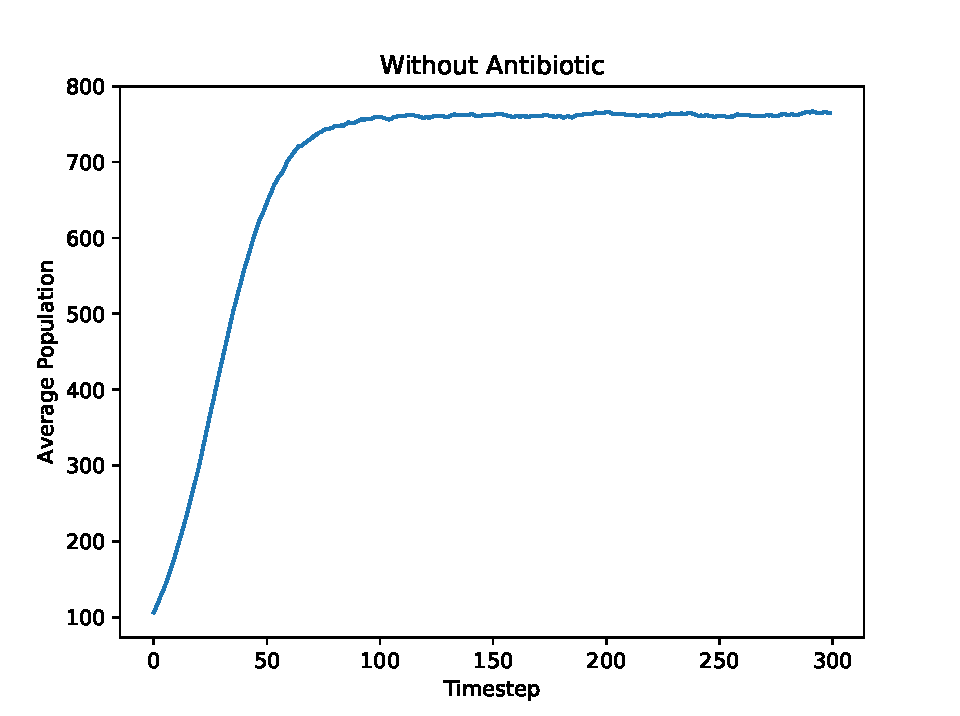
\includegraphics[width=0.8\linewidth]{fig/p2.pdf}
\caption{问题二结果}
\label{fig:p2}
\end{figure}

\begin{figure}[H]
\centering
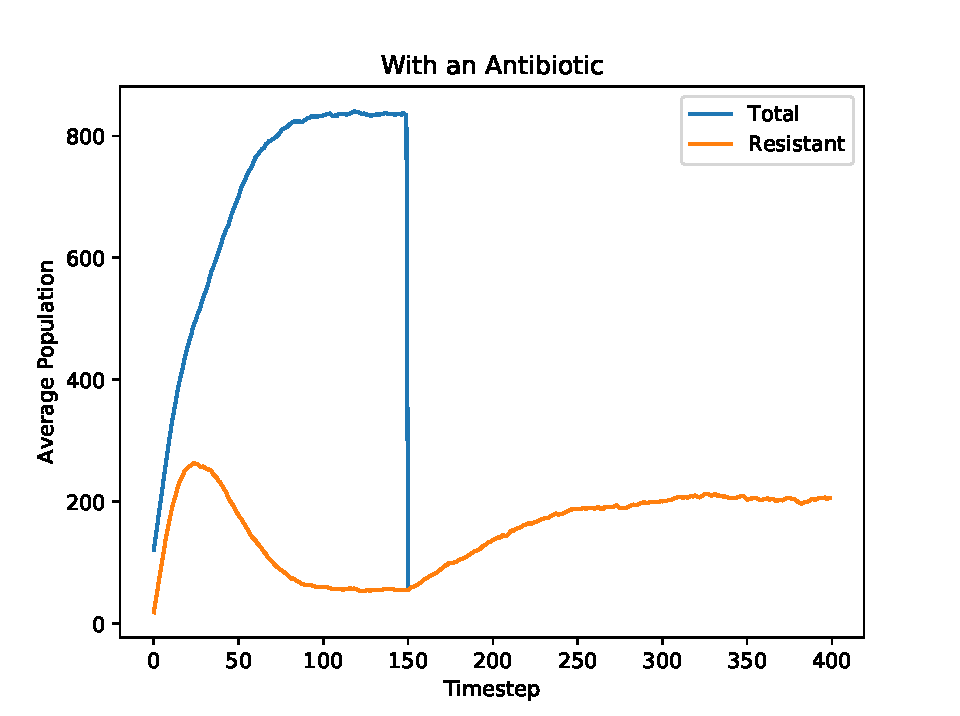
\includegraphics[width=0.8\linewidth]{fig/p5a.pdf}
\caption{问题五A结果}
\label{fig:p5a}
\end{figure}

\begin{figure}[H]
\centering
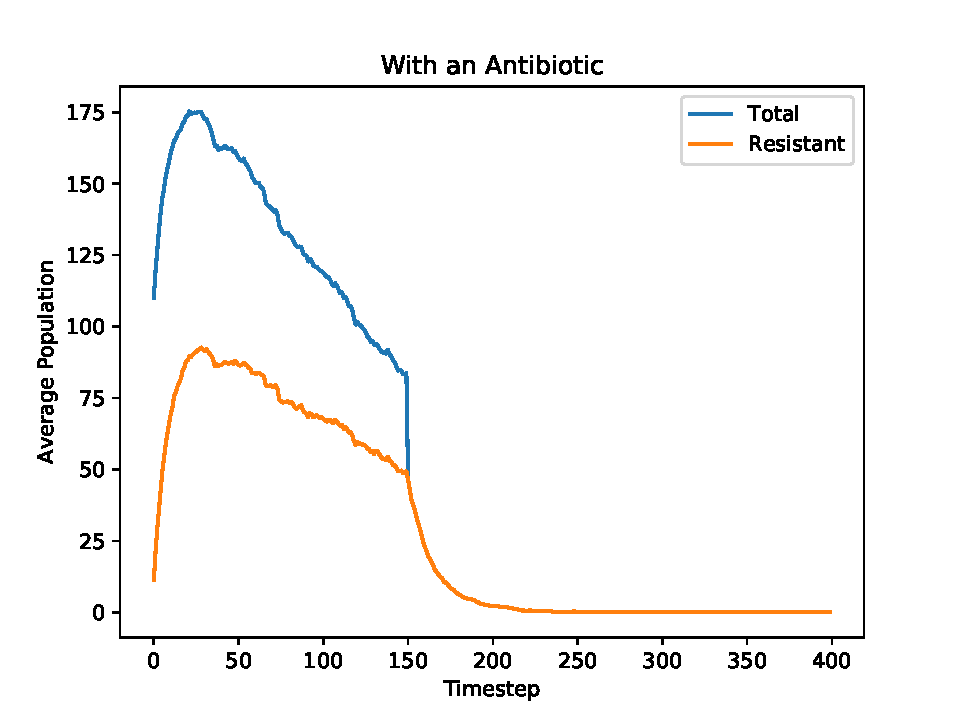
\includegraphics[width=0.8\linewidth]{fig/p5b.pdf}
\caption{问题五B结果}
\label{fig:p5b}
\end{figure}

\end{document}

% 实验提交内容
% 邮件主题,作业文件命名规范(学号、姓名) 学号+姓名+psX+vY
% 文档pdf格式(问题、求解思路、代码、注释、运行截图)
% 考虑健壮性、可读性
% 极端样例